REMOVED

\subsubsection{Methods}\hfill

\texttt{cityseer-api} \cite{simons_cityseer_2023} is used for computing centralities, land-use accessibilities, and mixed-use measures. The full workflow is available in the linked code repositories.

The preparation of the street network broadly entails the following steps:

\begin{enumerate}
\item The Madrid boundary is buffered by 10km prior to extracting the street network, so that the calculation of network centralities (within Madrid's boundary) is not impacted by edge-effects \cite{Gil2017}.
\item The source dataset necessitates splitting of lines where intersecting, with the implication that grade-separated crossings need to be stitched back together to maintain the separation of disconnected roadway segments. This was done through manual edits applied mainly to motorways (freeways). A limited number of network edits are also made where necessary for inner Madrid, though the source network is otherwise of a good quality. The original and edited versions of the network are available as Geopackage files in the aforementioned \texttt{madrid-ua-dataset} repository.
\item `Filler' nodes (nodes which do not represent intersections, therefor of degree 2) are removed, as are nodes representing short network stubs (e.g. driveways) and disconnected portions of the network.
\item The network is cast to its dual representation: primal street edges are split at their midpoints and are welded to adjacent (split) edges to create the new dual edges over which the metrics are computed. This process preserves the geometrical form of the network throughout, with distances in metres and angular deviation preserved.
\item Network centralities are computed for distances ranging from 200m to 10km using both \emph{metric distances} and \emph{geometric distances} (angular). Length weighted and segment (continuous) forms are also computed.
\end{enumerate}

\begin{figure}[ht]
\centering
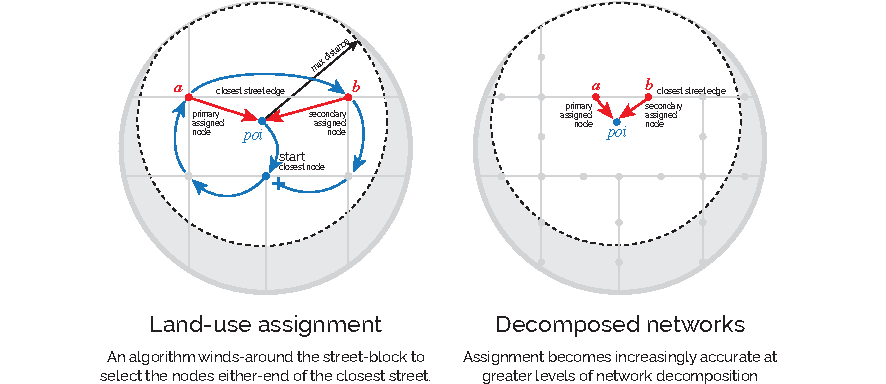
\includegraphics[width=\linewidth]{images/poi_assignment.pdf}
\caption{Street assignment of data points.}\label{fig:poi-assign}
\end{figure}

A winding algorithm "circles the block" to identify the adjacent street edge closest to each landuse location, with the landuse then assigned to the nodes on either side (Figure~\ref{fig:poi-assign}). The algorithms which measure distances to landuses can subsequently use either direction of approach when determining the final network distances relative to each point of analysis, which are the same nodes used for the calculation of network centralities. This closest-segment approach avoids situations where the nearest node may otherwise be located on the opposite side of an urban block. The use of network decomposition affords greater contextual precision when measuring distances and comparing metrics, though is not applied in this instance.

The preparation of the landuses data includes the following steps:

\begin{enumerate}
\item A landuse schema is extracted from the source Premises dataset, consisting of approximately 80 landuses.
\item Landuses are assigned to the street network based on the closest adjacent street edge, using a winding algorithm detailed in Figure~\ref{fig:poi-assign}.
\item Landuse accessibilities are computed relative to each node as detailed in Figure~\ref{fig:collapsing}. Distances are computed dynamically from the node to each landuse taking into account the direction of approach. This allows the determination of distances and facilitates the use of distance-weighted aggregation methods.
\item Mixed-uses are calculated using the landuse schema. Due to the richness of the schema a Hill Index of $q=0$ is used, subsequently referred to as \emph{Landuse Richness}.
\end{enumerate}

Whereas the Gini-Simpson diversity index \cite{Simpson1949} and Shannon information entropy \cite{Shannon1948} are commonly used, these have notable drawbacks. The Gini-Simpson diversity does not behave linearly with the addition of species, thus preventing comparisons for localised analysis \cite{Chao2014}. The Hill diversity index \cite{Hill1973, Jost2006, Tuomisto2010} is preferable because it quantifies true diversity as opposed to information or uncertainty, thus conferring a more intuitive mathematical behaviour. It further adheres to a replication principle, thus facilitating mathematically robust comparisons between locations.

A dynamic land-use aggregation workflow computes distances directly over the street network while taking the direction of approach into account (Figure~\ref{fig:collapsing}). The preservation of distances from each point of analysis to each accessible landuse allows for weighting by spatial impedances when calculating accessibilities and mixed-uses, thus conferring granular and spatially precise assessment of access to landuses from a given network node.

